% !TeX root = ../main.tex
% Add the above to each chapter to make compiling the PDF easier in some editors.

\chapter{Evaluation}\label{chapter:evaluation}
%------------------------------------------------------------------------
\section{Analysis}
In the following section we will conduct an analysis of our various numerical results
and benchmarks.
We will discuss the
particularites of the structure of these LP problems, and if there are any
patterns in their solution
process. This analysis is based on observing the statistical results we obtained from
running different solvers on these problems. This will provide us with insight
regarding the optimization of these problems.

We will also analyse and compare the time performance for our implementation solvers,
Umbra's revised simplex with the MPFI update variant, Cplex and HiGHS.


%------------------------------------------------------------------------
\subsection{Analysis JOB dataset}

\subsubsection{Structure and properties}
In  this subsection we will conduct an analysis the JOB dataset properties.

A opposed to what the linear programming research has dealt with, which is
very large problems, we are dealing with hundreds of small problems. The statistics
collected about the JOB dataset in the Table \ref{table_job_stats} prove this, since the LP size range is small, (number
of rules ranging from 1 to 19 and number of variables between 1 and 6).

Given the size of these LPs one might think the constraint matrices involved
are practically dense, however our results show differently. If we look at the densities
in the Table \ref{table_job_stats} we can see that the constraint matrix average density
for the JOB queries is around $0.6703$.

These matrices are represented
in the revised simplex algorithm by
sparse matrices but not as sparse as it would have been if the problem was large, i.e.
small matrices that are not small enough to be dense.

\subsubsection{Time efficiency}
From the table \ref{table_lps_hr_job}, we can see that the Tableau solver
outperforms the two other revised simplex solvers and Cplex. It records
the largest Query-Per-Hour metric, around $ 1.4 \texttt{billion}$ queries per hour.
The time profiles of the three solvers show that for the queries that have
an LP size less than 250 (we define the LP size as the product of the number 
of variables and the number of rules this LP has $\texttt{lp\_size} = m \times n$)
Tableau is the best out of the three. 
However, from $\texttt{lp\_size} \geq 250$ PFI outperforms the tableau method.
Meanwhile, the MPFI delivers the worst execution time out of the three solvers, for
this JOB dataset of small queries. 

Also, Cplex is slower than all other solvers for this dataset.

These results may be due to several reasons. We think most likely reason,
according to theoretical analysis of the functionalities of these solvers, and the documentation
of Cplex, is based on the small size of these LP problems.

\begin{itemize}
    \item Overhead of Cplex: Cplex, being a commercial solver, is designed to handle
    large-scale LPs. To do this, it incorporates many (in our case unnecessary) advanced techniques like 
    long initialization phases, presolving,
    where it attempts to simplify the LP, analyze it, identify special structures... While
    this can be highly beneficial for large and more complex problems, for small ones it 
    introduces unnecessary overhead.
    \item Simplicity of Tableau solver: our solver is very basic, skips unnecessary
    preprocessing or initialization. The bottleneck of the Tableau simplex solver
    is the Pivoting step, which includes row operations on dense matrices.
    For small problems, the data might fit entirely within the CPU cache, 
    making certain operations faster. The 1D dense matrix data structure may be a good 
    choice for this reason.
    \item Overhead of revised simplex methods: in the revised simplex method we start by
    preparing the sparse matrix format. This data structure offers a beneficial speedup 
    for larger sparser problems, but for small problems it represents an unnecessary 
    overhead, compared to the Tableau simplex, even though the latter uses a dense 
    representaion of the tableau, but in 1D vector, which may be more cache-friendly.
    The Revised Simplex method updates the matrix by enqueing an eta file to the pivots,
    but it still applies two basis multiplications BTRAN and FTRAN
    , which can be slower than the Pivoting operation of Tableau, especially for
     small problems.

\end{itemize}

It's worth noting that while the Tableau Simplex might be faster for some small LPs, 
it can be 
much slower than the Revised Simplex or CPLEX for larger or more complex problems. 
This is what we will discuss in  the next part of the analysis.

%------------------------------------------------------------------------
\subsection{Analysis of experiments on randomly generated LPs}
For small LP sizes, we observed that a basic implementation like tableau simplex
ouperform the revised simplex implementations as well as Cplex. However, for
larger LPs we come across other results. 
From figure \ref{fig:size_time_random_large} we see that Tableau does not scale well,
compared to revised simplex with PFI and MPFI update methods.

Also, starting from $\texttt{lp\_size} \geq 15,000$ approximately, we observe in Figure
\ref{cplex_vs_all_random_large} that Cplex starts outperforming our solvers.

\subsubsection{Why is highs so slow?}
using \texttt{linprog} from SciPy with HiGHS as a method can be 
slower than using the HiGHS interface directly, mainly due to the overhead, 
additional features and encapsulation.

\section{Results}
All the following results have been obtained on a system with the following settings:
\begin{itemize}
    \item OS: Ubuntu 22.04.1 LTS x86\_64
    \item Host: 82A2 Yoga Slim 7 14ARE05
    \item CPU: AMD Ryzen 7 4800U with Radeon Graphics (16) @ 1.800GHz
    \item GPU: AMD ATI 03:00.0 Renoir
    \item RAM: 10409MiB / 15363MiB
\end{itemize}

Presolve techniques are not used, the solvers assume an input of the form explained
in the UML graph \ref{fig:hierarchy} and in the format input as described
in the following section.

The computed optimal solutions have been validated using the scipy python library,
our solvers terminate and deliver correct optimum.

\subsubsection{Note on cache locality}
Through our experiments, we have noticed that if we call our C++ solvers
consecutively, this may affect the recorded exectuin times and thus make our benchmarks
unreliable or inaccurate. This may be due to cache locality: If the second solver is working
on data that was recently processed by the first solver, it might benefit from cache locality,
as some of the required data
might still be in the cache. This can lead to faster execution times for the second solver.
However, if the first solver used a significant amount of memory and displaced data relevant
to the second solver from the cache, then the second solver might experience cache misses.
Cache misses
can slow down the execution as the CPU has to fetch the required data from the main memory.
We detect varying results when we switch the order in which we call our solvers, and so
this effect is likely significant.
Our solution to avoid this is by isolating the solvers, and calling each one independently
(by commenting out any calls to the others). This is our approach to receive
accurate performance measures, and be able to compare the solvers reliably.

%------------------------------------------------------------------------
\subsection{Results on Query datasets}
The input files \texttt{TPCH}, \texttt{TPCDS}, and \texttt{JOB} contain packing
\gls{lp} problems. We have already established the mathematical derivation of how
these query-related packing
\gls{lp} problems are generated in \ref{section:cardinality-estimate}.

The \texttt{lp.txt} file is structured for machine readability.
In this format, each line represents a single \gls{lp}. The line starts with
the number of rules in that problem. For each rule, the number of entries in
the coefficient matrix is specified first, followed by pairs of values:
the column number and the coefficient. This is convenient to parse the entries
and then populate our sparse matrix representation quite efficiently.

\begin{lstlisting}
lp:
8 2 0 0.0540277 2 0.0540277 ...
\end{lstlisting} \label{format_input}

\begin{table}[!htb]
    \centering
    \caption{Benchmarks and number of queries.}
    \begin{tabular}{|l|l|}
        \hline
        Benchmark                                & Number of Queries \\
        \hline
        JOB \parencite{10.14778/2850583.2850594} & 2230              \\
        TPC-H \parencite{tpch}                   & 16                \\
        TPC-DS \parencite{tpcds2022}             & 148               \\
        \hline
    \end{tabular}
    \label{job_tpch_tpcds}
\end{table}

\subsubsection{The JOB dataset results}
In the table \ref{table_job_stats} are some important statistical finds following our
experiments with the JOB dataset.
This is the largest dataset of all three query datasets. It contains duplicated queries so we
perform a removal of the duplicated LPs before. We collect the data and perform plotting and data summary
using R scripts.

\begin{figure}[!htb]
    \centering
    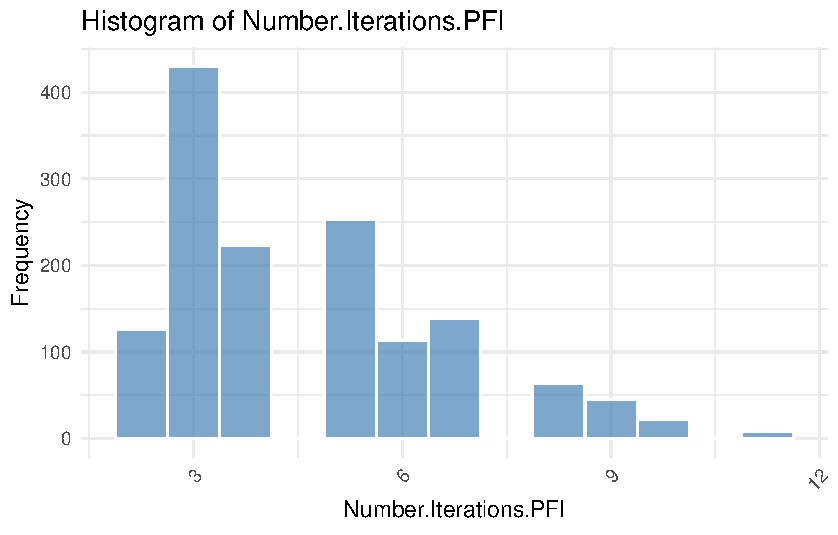
\includegraphics[width=\textwidth]{figures/histo_iter_pfi.pdf}
    \caption{Boxplot for number of iterations for PFI for JOB dataset}
    \label{fig:num_iter_boxplot_pfi_job}
\end{figure}

\begin{figure}[!htb]
    \centering
    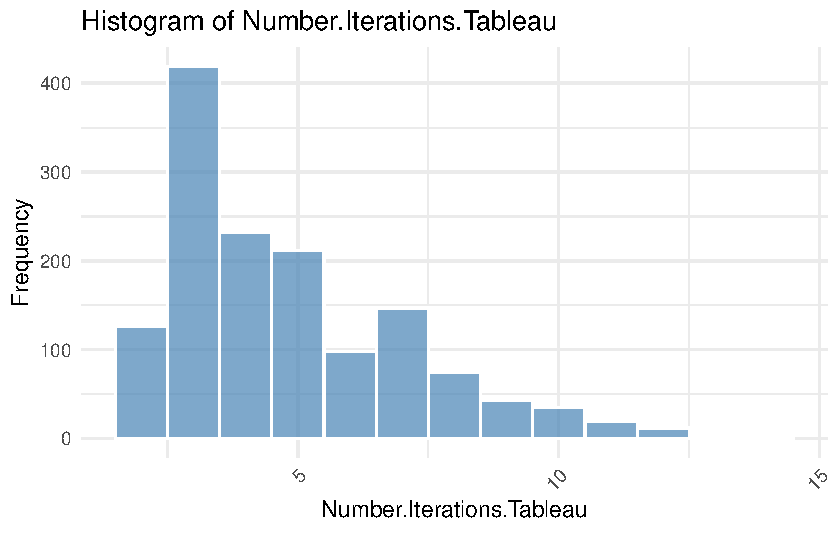
\includegraphics[width=\textwidth]{figures/histogram_iter_tableau.pdf}
    \caption{Boxplot for number of iterations for Tableau for JOB dataset}
    \label{fig:num_iter_boxplot_tableau_job}
\end{figure}


\begin{figure}[!htb]
    \centering
    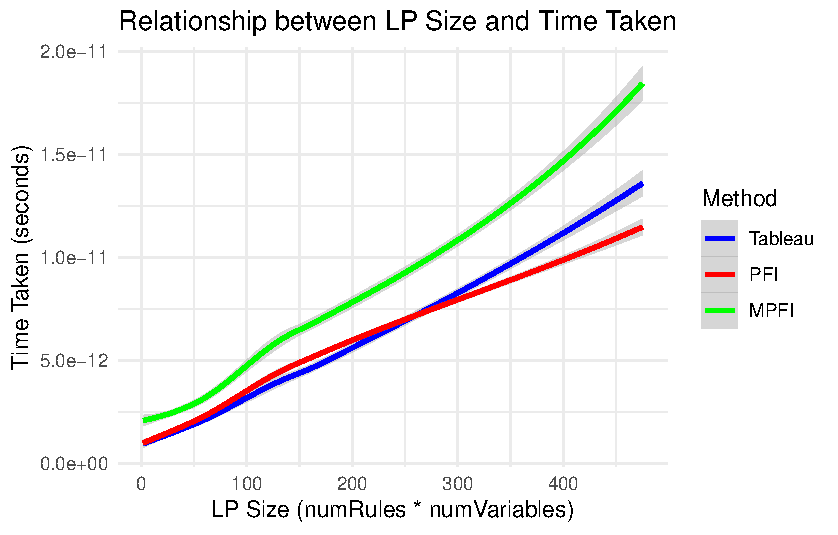
\includegraphics[width=\textwidth]{figures/lp_size_vs_time_job.pdf}
    \caption{Relation between LP size and time for the 3 simplex solvers for JOB dataset.}
    \label{fig:lp_size_vs_time_job}
\end{figure}

\begin{table}[!htb]
    \centering
    \caption{Statistics about JOB dataset}
    \begin{tabular}{lrrrr}
        \toprule
        Variable                  & Min    & Median  & Mean    & Max     \\
        \midrule
        LP size                   & 2.00   & 54.00   & 94.56   & 475.00  \\
        Number of Rules           & 1.000  & 6.000   & 7.037   & 19.000  \\
        Number of Variables       & 1.00   & 3.00    & 3.07    & 6.00    \\
        Constraint Matrix Density & 0.3684 & 0.6667  & 0.6703  & 1.0000  \\
        Solution Time Scipy       & 650    & 931     & 959     & 1802    \\
        Solution Time Cplex       & 97.04  & 184.06  & 190.66  & 415.56  \\
        Solution Time Tableau     & 2.00   & 4.00    & 12.15   & 4274.00 \\
        Solution Time PFI         & 2.000  & 6.000   & 8.316   & 65.000  \\
        Solution Time MPFI        & 1.000  & 4.000   & 5.517   & 68.000  \\
        Number Iterations Tableau & 2.000  & 4.000   & 4.829   & 14.000  \\
        Number Iterations PFI     & 2.000  & 4.000   & 4.621   & 11.000  \\
        Number Iterations MPFI    & 2.000  & 4.000   & 4.671   & 13.000  \\
        Optimal Value             & 0.3188 & 20.6702 & 21.8575 & 42.1804 \\
        \bottomrule
    \end{tabular}
    \label{table_job_stats}
\end{table} 

This is our results:
\begin{table}[!htb]
    \centering
    \caption{Number of LPs or Queries Solved by Hour for the JOB dataset}
    \begin{tabular}{l|r}
        \toprule
        Method                     & Number of LPs/Queries \\
        \midrule
        Revised Simplex MPFU Umbra & 906,607,929           \\
        Tableau Simplex            & 1,400,923,787         \\
        Revised Simplex PFI        & 1,287,140,216         \\
        Scipy (method highs)       & 4,069,108             \\
        Cplex                      & 17,849,851            \\
        \bottomrule
    \end{tabular}
    \label{table_lps_hr_job}
\end{table} 



\subsubsection{TPC-DS results}

\begin{figure}[!htb]
    \centering
    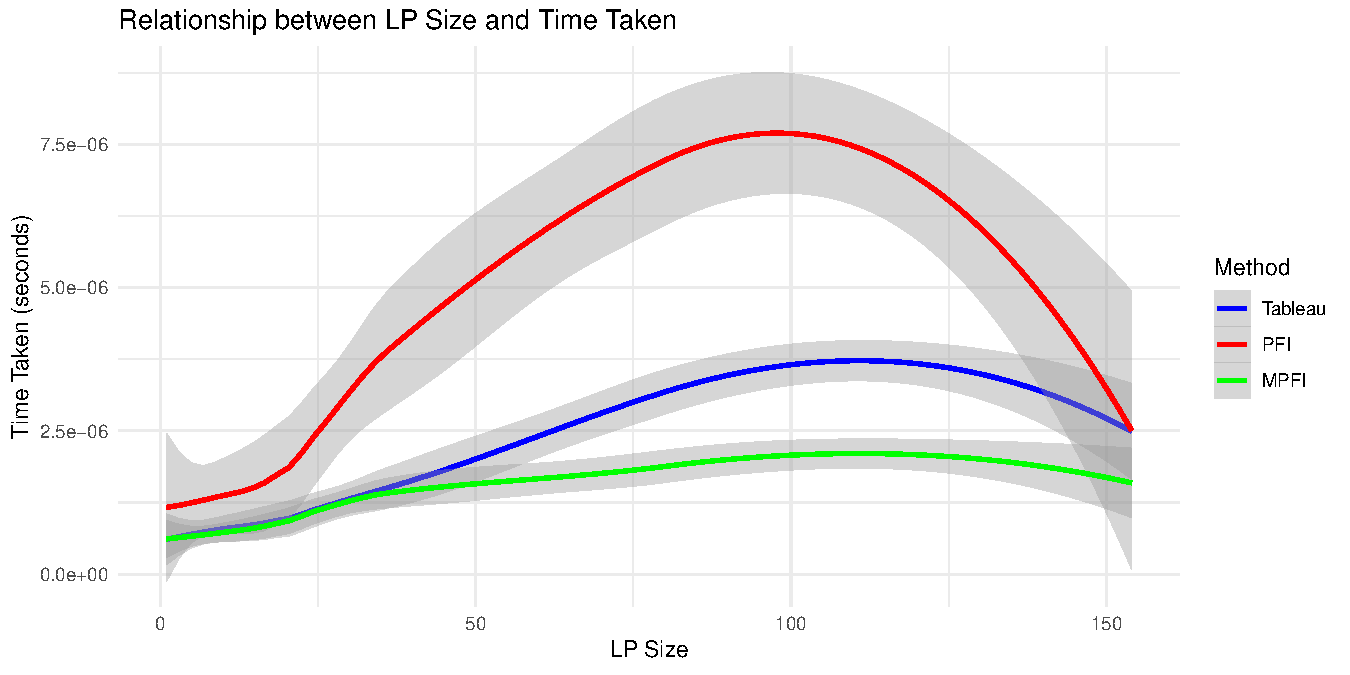
\includegraphics[width=\linewidth]{figures/methods_time_tpcds.pdf}
    \caption{A graph comparing the time performance of two of
    our solvers with scipy solver solving the tpcds dataset}
    \label{fig:methods_time_tpcds}
\end{figure}

\begin{figure}[!htb]
    \centering
    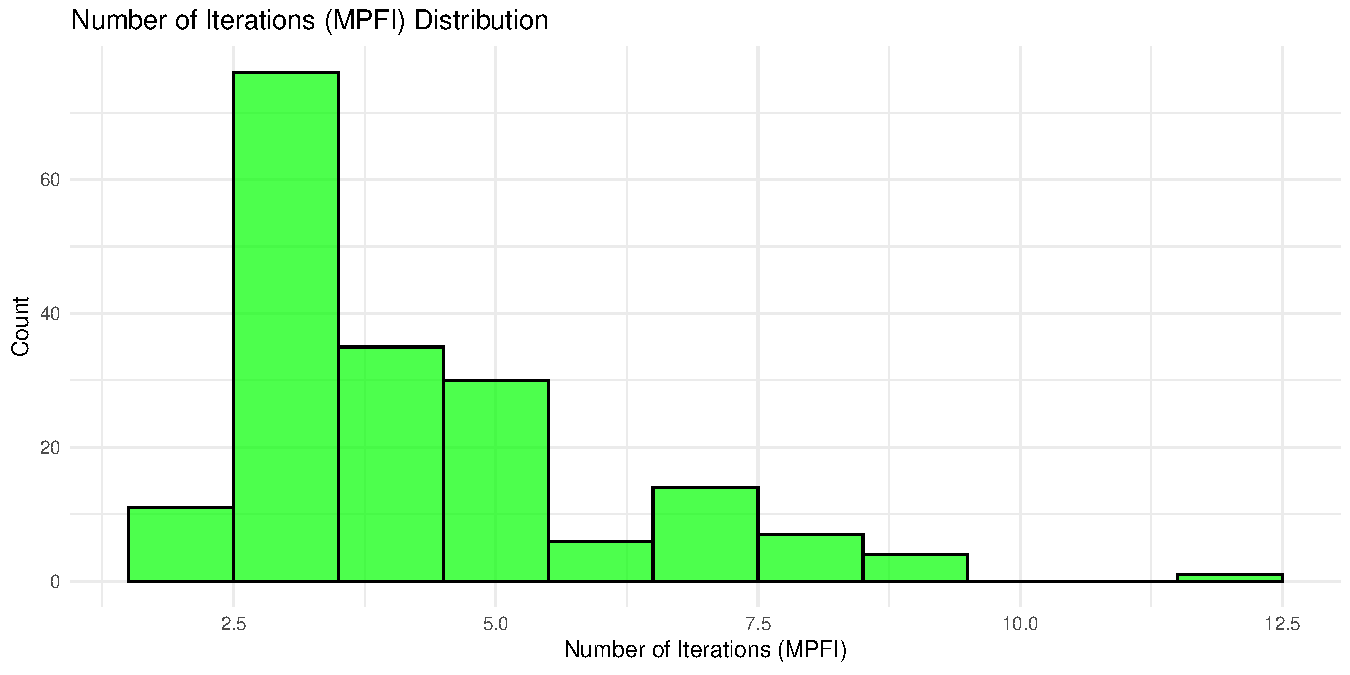
\includegraphics[width=\linewidth]{figures/num_iter_tpcds_mpfi.pdf}
    \caption{Boxplot for number of iterations for MPFI for TPCDS dataset}
    \label{fig:num_iter_tpcds_mpfi}
\end{figure}

\begin{figure}[!htb]
    \centering
    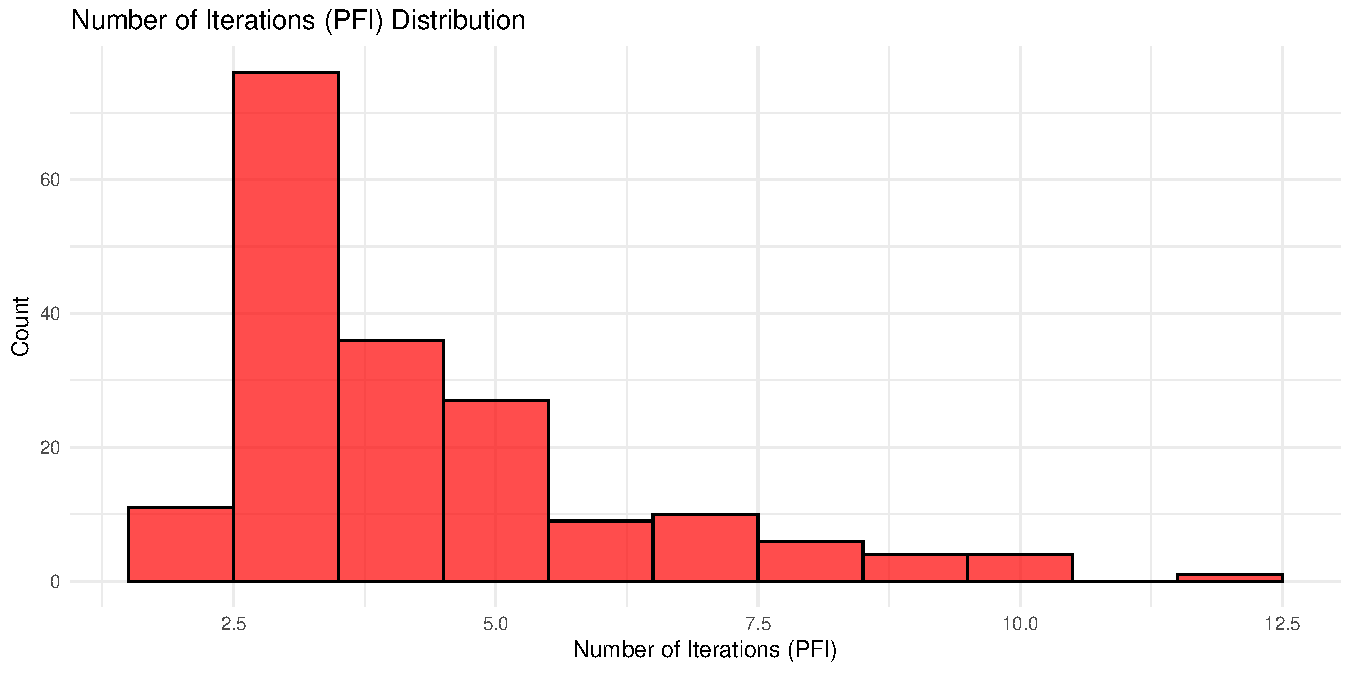
\includegraphics[width=\linewidth]{figures/num_iter_pfi_tpcds.pdf}
    \caption{Boxplot for number of iterations for PFI for TPCDS dataset}
    \label{fig:num_iter_pfi_tpcds}
\end{figure}


\subsubsection{TPC-H results}


%------------------------------------------------------------------------
\subsection{Results on randomly generated LPs}
We also test our solvers alongside Cplex, on packing LPs generated randomly.

We use a python script as a generator for packing linear programming (LP) problems.
It creates LP problem instances
based on the specified number of rules and variables.
For each rule, a random number of entries, ranging from 1 to
the total number of variables, is determined.
For every entry in a rule, a unique column number is randomly selected from
the available variables, ensuring that the same column is not used more than once for
the same rule. A random coefficient, between 0.1 and 1.0, is then assigned to
this column. The entire LP problem is represented as a space-separated string,
where the first entry denotes the number of rules, followed by the number of
entries for each rule, and then the column-coefficient pairs.
The main part of
the script generates a series of such LP problems, incrementally increasing the
number of rules and variables for each problem, and writes them to a text file.
This is how we get our randomly generated packing LPs with increasing sizes in the same format
as the query datasets.

We run our solvers, and also Cplex on this dataset, which provide us with numerical results
in the figures: \ref{fig:time_vs_size_random}, \ref{fig:lps_per_hour_random}, \ref{fig:size_time_random_large},
\ref{fig:speedup_cplex_less_1000.pdf}, and \ref{fig:speedup_cplex_random.pdf}.

We want to
explore those results to investigate how these solvers scale, and if the speedup
they provide is still substantial at larger LPs.


\begin{figure}[!htb]
    \centering
    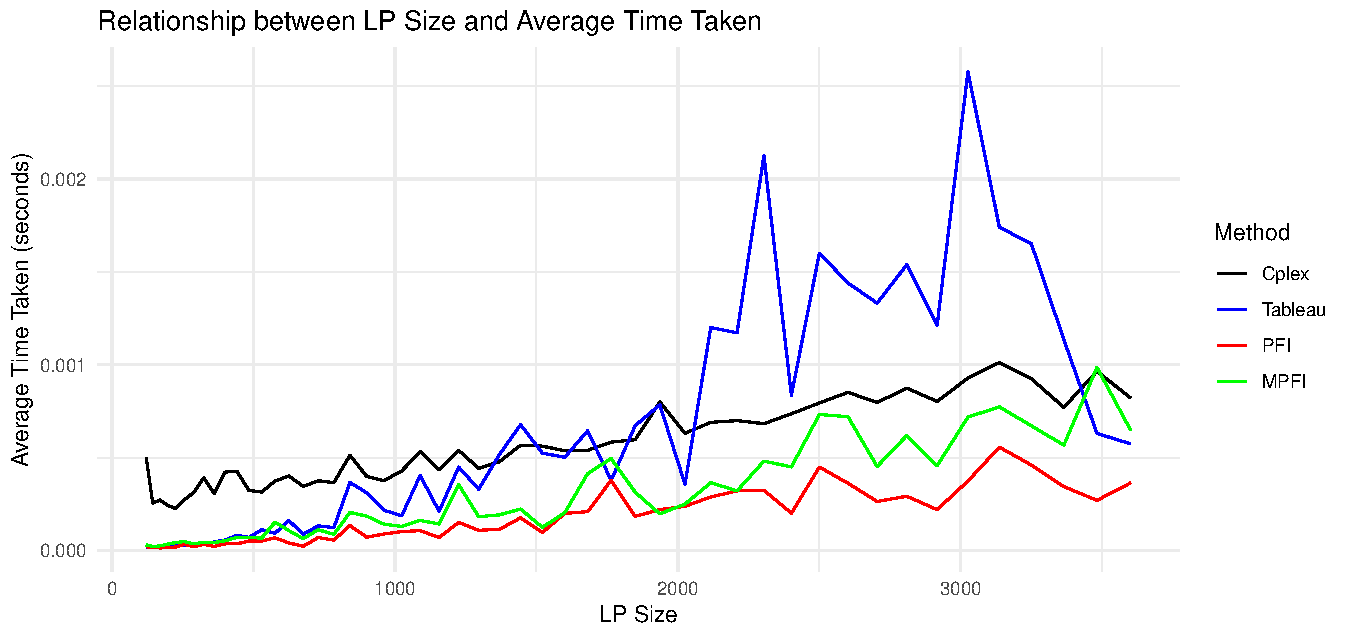
\includegraphics[width=0.8\textwidth]{figures/time_vs_size_random.pdf}
    \caption{Relation between LP size and time for the 3 simplex solvers and Cplex for randomly generated
        dataset with increasing LP size.}
    \label{fig:time_vs_size_random}
\end{figure}


\begin{table}[!htb]
    \centering
    \caption{Number of LPs Solved by Hour for the randomly generated dataset}
    \begin{tabular}{l|r}
        \toprule
        Method                     & Number of LPs \\
        \midrule
        Revised Simplex MPFU Umbra & 13,520,349    \\
        Tableau Simplex            & 6,963,530     \\
        Revised Simplex PFI        & 24,352,331    \\
        Cplex                      & 6,666,083     \\
        \bottomrule
    \end{tabular}
    \label{fig:lps_per_hour_random}
\end{table} 

We get the time profile in Figure \ref{fig:time_vs_size_random}.
We want to see the further evolution of this time profile, so we increase the number of generated LPs
and explore larger LPs, see Figure \ref{fig:size_time_random_large}.

\begin{figure}[!htb]
    \centering
    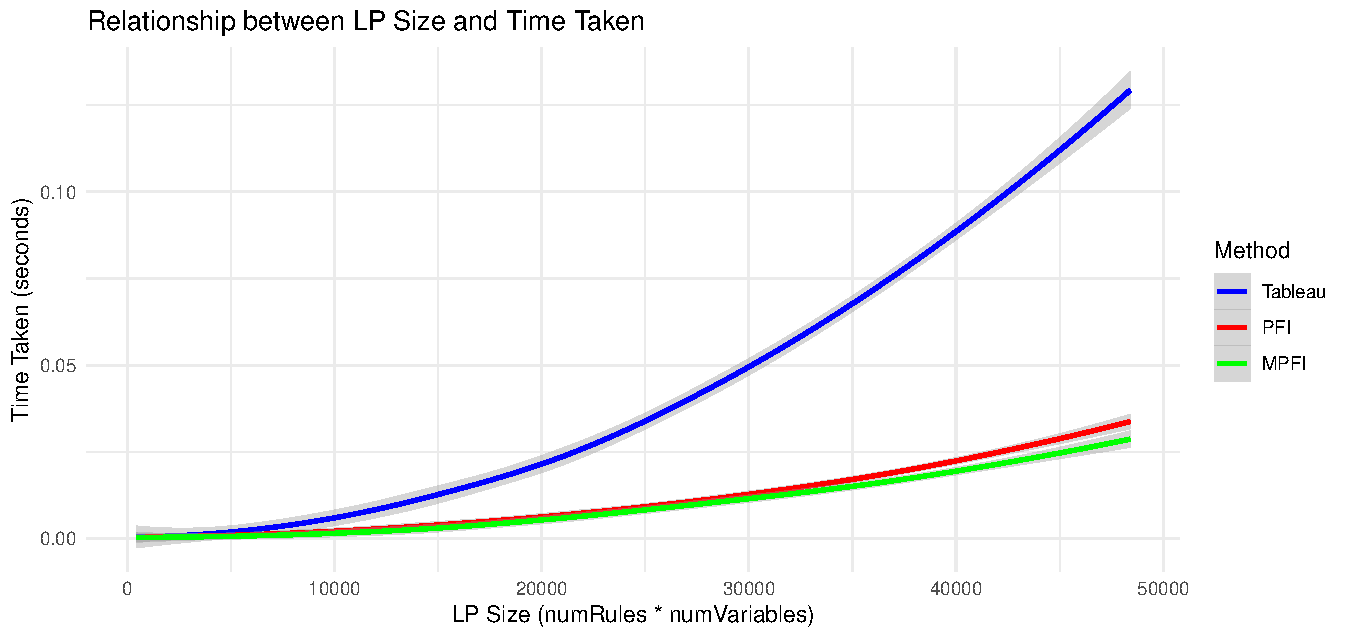
\includegraphics[width=\linewidth]{figures/size_time_random_large.pdf}
    \caption{Relation between LP size and time for the 3 simplex solvers for the randomly generated
        dataset with increasing LP size ranging up to 220 rules and 220 variables.}
    \label{fig:size_time_random_large}
\end{figure}

\begin{figure}[p]
    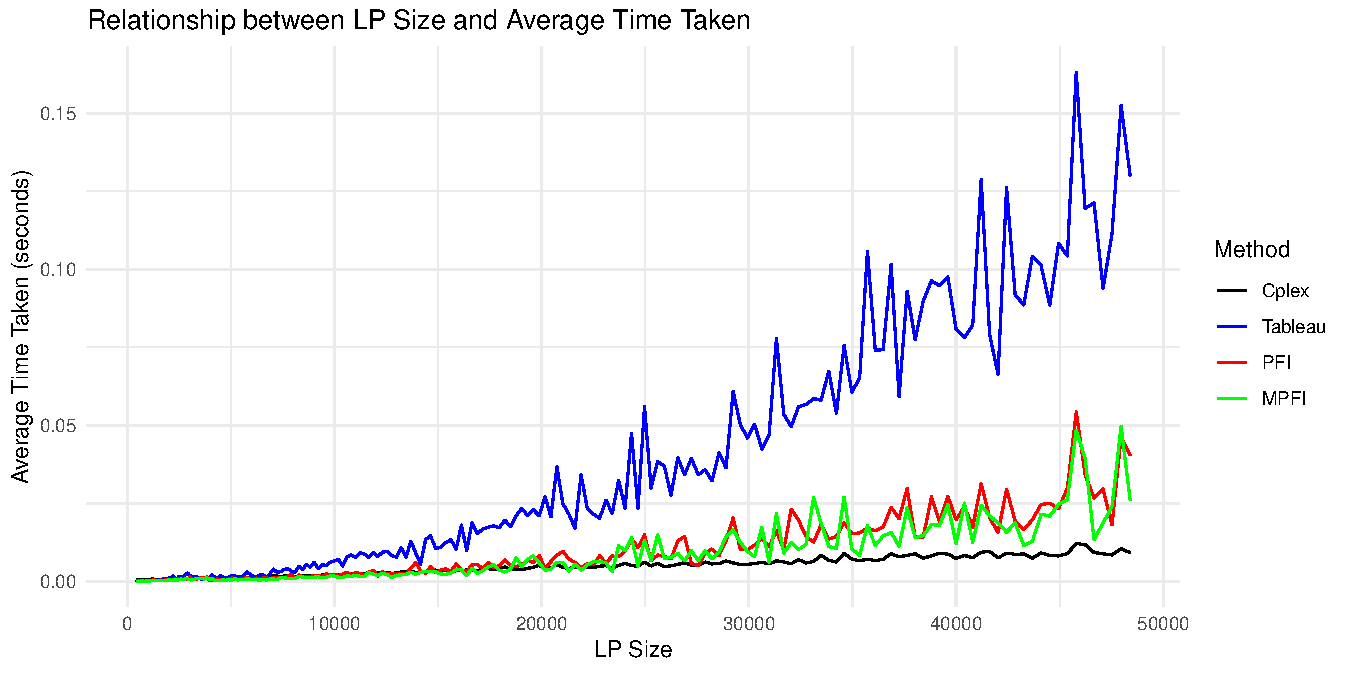
\includegraphics[width=0.8\paperwidth, height=\paperheight, keepaspectratio]{figures/cplex_vs_all_random_large.pdf}
    \caption{Relation between LP size and time for the 3 simplex solvers with CPLEX randomly generated
        dataset with increasing LP size ranging up to 220 rules and 220 variables.}
    \label{cplex_vs_all_random_large}
\end{figure}

\begin{figure}[!htb]
    \centering
    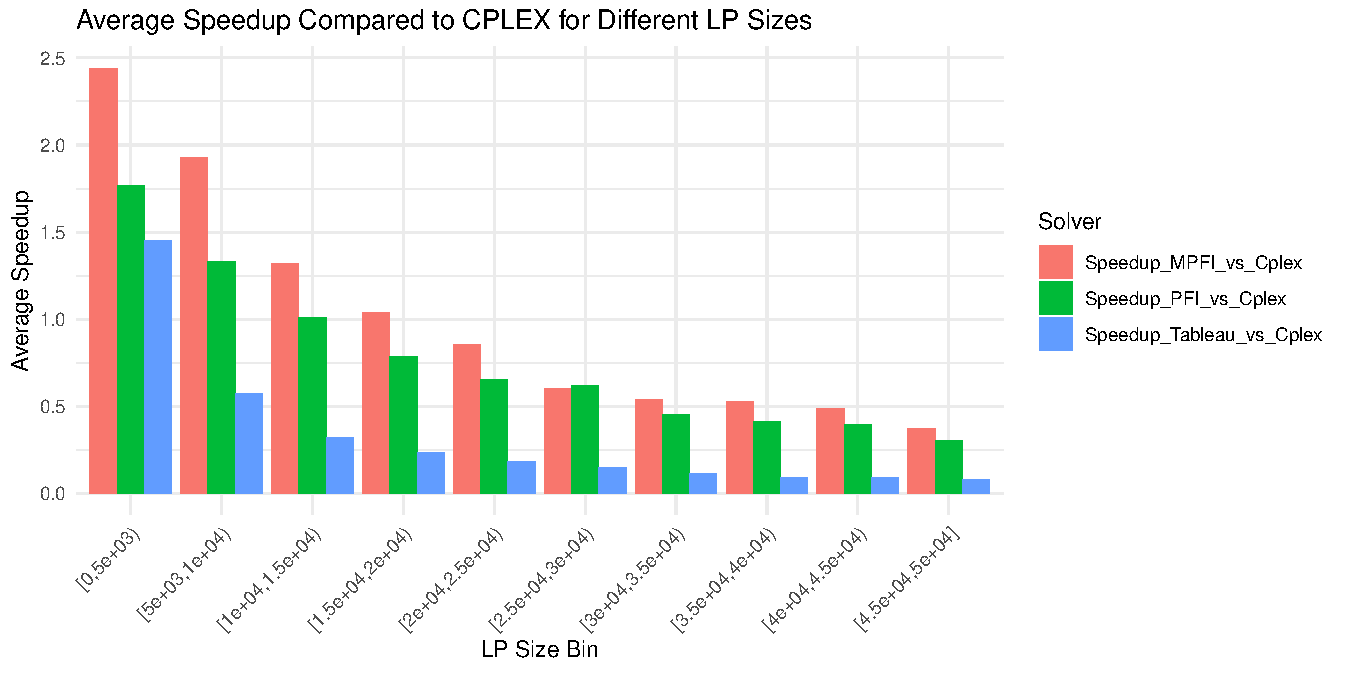
\includegraphics[width=\linewidth]{figures/speedup_vs_cplex_random_200.pdf}
    \caption{Speedup of the three solvers (how many times faster they are) compared to CPLEX for
        the randomly generated dataset for increasing LP size}
    \label{fig:speedup_cplex_random.pdf}
\end{figure}

\begin{figure}[!htb]
    \centering
    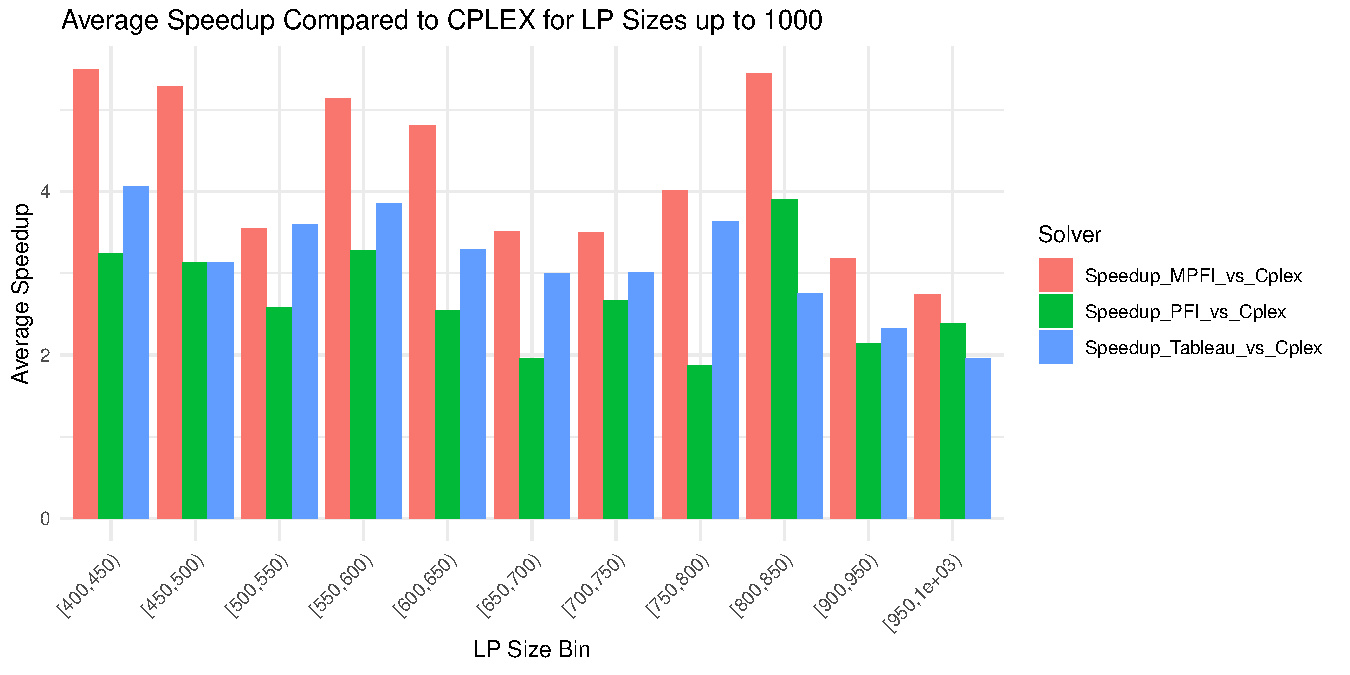
\includegraphics[width=\linewidth]{figures/speedup_cplex_less_1000.pdf}
    \caption{Speedup of the three solvers (how many times faster they are) compared to CPLEX for
        the randomly generated dataset for the LP size up to 1000}
    \label{fig:speedup_cplex_less_1000.pdf}
\end{figure}

%------------------------------------------------------------------------


\section{Limitations}

\section{Future Work}
\subsection{Forrest-Tomlin update form}
The Forrest-Tomlin (FT) update enhances efficiency in the
revised simplex method by modifying the LU decomposition of the basis matrix B.
This update efficiently handles the BTRAN and FTRAN systems.
It begins with the basis matrix update equation:

\[
    \bar{B} = B + (a_q - B e_p) e_p^T \Rightarrow L^{-1} \bar{B} = U + (L^{-1}a_q - U e_p) e_p^T = U'
\]

Here, \(U'\) is a spiked upper factor.
The FT update restores triangularity to \(U'\) by using row transformations.
It employs a row eta matrix \(R\) such that \(\bar{U} = R^{-1}U'\). 
The row eta matrix \(R\) can be expressed as \(R = I + e_p r^T\) and \(R^{-1} = I - e_p r^T\), where \(r\) is calculated as \(r^T = \bar{u}_p^T U^{-1}\).

The representation of \(\bar{U}\) is obtained by inserting \(r\) and 
adjusting the sequence of eta vectors, pivotal entries, and pivotal indices. 
This ensures that \(\bar{U}\) remains invertible.

Combining \(\bar{B} = LU'\) and \(\bar{U} = R^{-1}U'\), we obtain the 
updated representation of the basis matrix and its inverse:

\[
    \bar{B} = LR \bar{U} \quad \text{and} \quad \bar{B}^{-1} 
    = \bar{U}R^{-1}L^{-1}
\]

After \(k\) updates, the basis matrix \(B_k\) and its inverse can 
be expressed as:

\[
    B_k = LR_1R_2 \ldots R_kU_k \quad \text{and} \quad B_k^{-1} 
    = U_k^{-1}R_k^{-1}R_{k-1}^{-1} \ldots R_2^{-1}R_1^{-1}L^{-1}
\]

This representation efficiently handles updates in the revised simplex method.

